\documentclass[11pt,letterpaper,notitlepage]{report}
\usepackage[latin1]{inputenc}
\usepackage{amsmath}
\usepackage{amsfonts}
\usepackage{amssymb}
\usepackage{fancyhdr}
\newcommand{\field}[1]{\mathbb{#1}}
\renewcommand{\labelenumi}{\alph{enumi})}
\usepackage{tikz}
\usepackage{fancybox}
\title{Minesweeper Solver Analysis}
\author{Brian Stack, bis12@case.edu}
\date{\today}
\usepackage[small,bf]{caption}
\usepackage{subfigure}
\usepackage{wrapfig}
\usepackage{fullpage}
\usepackage{tikz}
\usepackage{tikz-qtree}



\begin{document}
\maketitle
\section*{Analysis of Game}
\begin{enumerate}
\item 
\begin{align*}
C = \{ (V_1, V_2) &= V_1 + V_2 = 1,\\
       (V_3, V_4) &= V_3 + V_4 = 1,\\
       (V_1, V_2, V_3, V_4, V_5) &= V_1 + V_2 + V_3 + V_4 + V_5 = 2\}
\end{align*}
\item Any nodes marked as Imp are impossible states. It does provide an optimal next choice, which is $V_5$.
\begin{center}
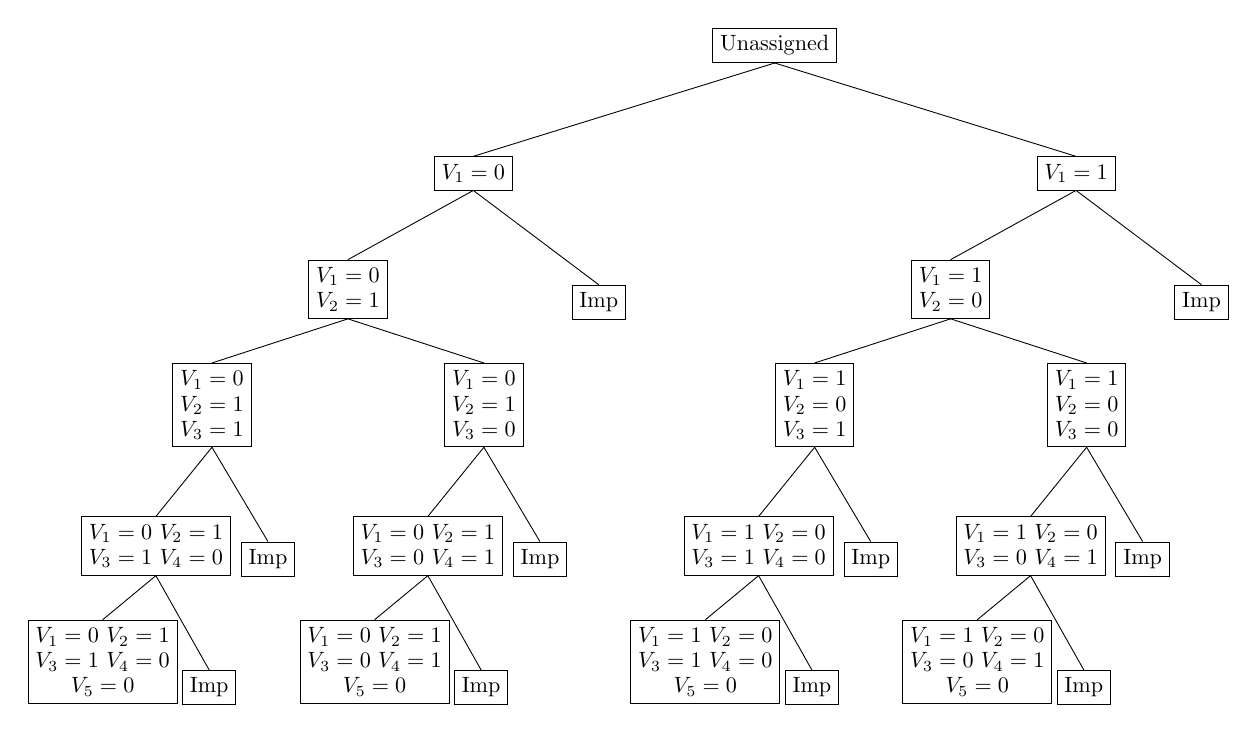
\begin{tikzpicture}[scale=0.8]
\tikzset{level distance=58pt}
\tikzstyle{every node}=[rectangle,draw]
\Tree [.Unassigned [.{$V_1 = 0$}
[.\shortstack{$V_1 = 0$\\$V_2 = 1$} 
[.\shortstack{$V_1 = 0$\\$V_2 = 1$\\$V_3 = 1$} 
[.\shortstack{$V_1 = 0$ $V_2 = 1$\\$V_3 = 1$ $V_4 = 0$} [.\shortstack{$V_1 = 0$ $V_2 = 1$\\$V_3 = 1$ $V_4 = 0$\\$V_5 = 0$} ] [.Imp ]] 
[.Imp ] ] 
[.\shortstack{$V_1 = 0$\\$V_2 = 1$\\$V_3 = 0$} 
[.\shortstack{$V_1 = 0$ $V_2 = 1$\\$V_3 = 0$ $V_4 = 1$} [.\shortstack{$V_1 = 0$ $V_2 = 1$\\$V_3 = 0$ $V_4 = 1$\\$V_5 = 0$} ] [.Imp ] ] 
[.Imp ] ] ]
[.Imp ]
] [.{$V_1 = 1$}
[.\shortstack{$V_1 = 1$\\$V_2 = 0$} 
[.\shortstack{$V_1 = 1$\\$V_2 = 0$\\$V_3 = 1$} 
[.\shortstack{$V_1 = 1$ $V_2 = 0$\\$V_3 = 1$ $V_4 = 0$} [.\shortstack{$V_1 = 1$ $V_2 = 0$\\$V_3 = 1$ $V_4 = 0$\\$V_5 = 0$} ] [.Imp ]] 
[.Imp ] ] 
[.\shortstack{$V_1 = 1$\\$V_2 = 0$\\$V_3 = 0$} 
[.\shortstack{$V_1 = 1$ $V_2 = 0$\\$V_3 = 0$ $V_4 = 1$} [.\shortstack{$V_1 = 1$ $V_2 = 0$\\$V_3 = 0$ $V_4 = 1$\\$V_5 = 0$} ] [.Imp ] ] 
[.Imp ] ] ]
[.Imp ]
] ] 
\end{tikzpicture}
\end{center}
\item All four possibilities are enumerated below\\
\begin{tabular}{ccccc}
$V_1$&$V_2$&$V_3$&$V_4$&$V_5$\\\hline
0&1&1&0&0\\
0&1&0&1&0\\
1&0&1&0&0\\
1&0&0&1&0
\end{tabular}
\item $V_5$ cannot possibly reveal a mine because in no possible configuration does it contain one. Therefore $V_5$ is the safest.
\item The tree is 5 levels deep (same as the number of variables), and so the runtime is $\Theta(2^n)$ where $n$ is the number of variables.
\end{enumerate}
\section*{Observations on Solutions}
\begin{enumerate}
\item To make a choice, my agent first updates its state from the game, then runs a backtracking search to generate a list of all possible configurations of the current variables.  It then sums up the values of each variable by adding 1 to its sum if it is a mine in one of the possible configurations. At this point, the lowest valued choice is selected, and any that have a value equal to the length of the list of configurations are flagged as mines.
\item There is no way that I know of for a local search agent to know it has found all of the solutions to a problem without checking every solution.This however, would make this an exhaustive search, and would no longer be a ``local'' search.  Therefore, my local search implementation does not always move the same as the optimal backtracking search because it sometimes misses possible solutions.  When it does find all of the possible configurations of mines, it does make the same selection as backtracking because the selections process once the list of configurations has been generated is identical.  My implementation of local search is a random restart hill climbing search and is run multiple times over again with different starting points in an attempt to find all of the solutions.
\item Backtracking search will always find all solution that exist, whereas a local search has no guarantee that this will occur.  Therefore whenever possible, backtracking search would be the advisable option to solve this sort of problem.  However, when the number of variables and constraints gets very large, backtracking search cannot manage it, and in this case, a local search will have a better chance of finding the solutions. Backtracking search explored every valid node, whereas local search clearly will not traverse every path down the tree.  So far as memory and time costs go, local search is more efficient, but you pay for it in completeness.
\end{enumerate}
\end{document}





